
\documentclass[letterpaper, reqno,11pt]{article}
\usepackage[margin=1.0in]{geometry}
\usepackage{color,latexsym,amsmath,amssymb}
\usepackage{fancyhdr}
\usepackage{amsthm}
\usepackage[linesnumbered,lined,boxed,commentsnumbered,noend,noline]{algorithm2e}
\usepackage{dsfont}
\usepackage{graphicx}
\usepackage{hyperref}
\usepackage{bbm}
\usepackage{enumitem}
\usepackage[numbers]{natbib}
\usepackage{framed}
\usepackage{titling}
\usepackage{subcaption}
\usepackage[dvipsnames]{xcolor}
\usepackage{tikz}

\tikzset{invclip/.style={clip,insert path={{[reset cm]
  (-16383.99999pt,-16383.99999pt) rectangle (16383.99999pt,16383.99999pt)}}}}

\allowdisplaybreaks

\newcommand{\RR}{\mathbb{R}}
\newcommand{\CC}{\mathbb{C}}
\newcommand{\ZZ}{\mathbb{Z}}
\newcommand{\QQ}{\mathbb{Q}}
\newcommand{\NN}{\mathbb{N}}
\newcommand{\FF}{\mathbb{F}}
\newcommand{\PP}{\mathbb{P}}
\newcommand{\EE}{\mathbb{E}}
\newcommand{\LL}{\mathbb{L}}
\newcommand{\TT}{\mathbb{T}}
\DeclareMathOperator{\conv}{conv}
\DeclareMathOperator{\charcone}{char.cone}
\DeclareMathOperator{\STAB}{STAB}
\DeclareMathOperator{\Down}{Down}
\DeclareMathOperator{\lca}{lca}
\DeclareMathOperator{\ex}{ex}
\DeclareMathOperator{\Span}{span}
\DeclareMathOperator{\T}{T}
\DeclareMathOperator{\F}{F}
\DeclareMathOperator{\shP}{\# P}
\DeclareMathOperator{\shSAT}{\# SAT}
\DeclareMathOperator{\shDNF}{\# DNF}
\DeclareMathOperator{\DNF}{DNF}
\DeclareMathOperator{\Poly}{P}
\DeclareMathOperator{\CNF}{CNF}
\DeclareMathOperator{\SAT}{SAT}
\DeclareMathOperator{\BPP}{BPP}
\newcommand\mycommfont[1]{\ttfamily\textcolor{blue}{#1}}
\SetCommentSty{mycommfont}
\begin{document}
\pagenumbering{arabic}
\title{Lectures on Uniform Generation and Approximate Counting}
\author{Yuchong Pan}
\date{\today}
\newtheorem{theorem}{Theorem}
\newtheorem{lemma}[theorem]{Lemma}
\newtheorem{proposition}[theorem]{Proposition}
\newtheorem{corollary}[theorem]{Corollary}
\newtheorem{fact}[theorem]{Fact}
\newtheorem{claim}{Claim}
\newtheorem{exercise}{Exercise}
\theoremstyle{definition}
\newtheorem{definition}[theorem]{Definition}
%\maketitle
%

\begin{framed}
\noindent{\bf 6.842 Randomness and Computation} \hfill \thedate
\begin{center}
\Large{\thetitle}
\end{center}
\noindent{\em Lecturer: Ronitt Rubinfield} \hfill {\em Scribe: \theauthor}
\end{framed}

\section{Uniform Generation for DNF}

A \emph{DNF formula} is a Boolean formula that consists of ``OR of ANDs'', e.g., $\varphi(x_1, x_2, x_3) = x_1 \overline{x_2} \vee \overline{x_1} x_3$. The task is to output a random satisfying assignment to a DNF formula, uniformly over all satisfying assignments.

Consider the special case with only one conjunction. We can satisfy literals in the conjunction, and set the others randomly. For instance, for $\varphi(x_1, x_2, x_3) = x_1 \overline{x_2}$, we set $x_1 = \T, x_2 = \F$, and set $x_3 \in \{ \T, \F \}$ uniformly.

Now consider the two conjunction case, e.g., $\varphi(x_1, x_2, x_3) = x_1 x_2 \vee x_3$. We give an algorithm attempt in Algorithm \ref{alg:2-conj}. However, two problems arise, as illustrated in Figure \ref{fig:2-conj}. Firstly, conjunctions have different numbers of assignments. Secondly, some assignments can be chosen in multiple ways. In particular, using Algorithm \ref{alg:2-conj}, the probability that TTF is chosen is $1/2 \cdot 1/2 = 1/4$, the probability that TTT is chosen is $1/2 \cdot 1/2 + 1/2 \cdot 1/4 = 3/8$, and that the probability that each of TFT, FTT, FFT is chosen is $1/2 \cdot 1/4 = 1/8$.

\begin{algorithm}
  pick $i \in \{ 1, 2 \}$ uniformly \\
  set variables in conjunction $i$ to T \label{line:conj} \\
  set others uniformly
  \caption{An algorithm attempt of uniform generation for DNF with 2 conjunctions.}
  \label{alg:2-conj}
\end{algorithm}

\begin{figure}[h]
  \centering
  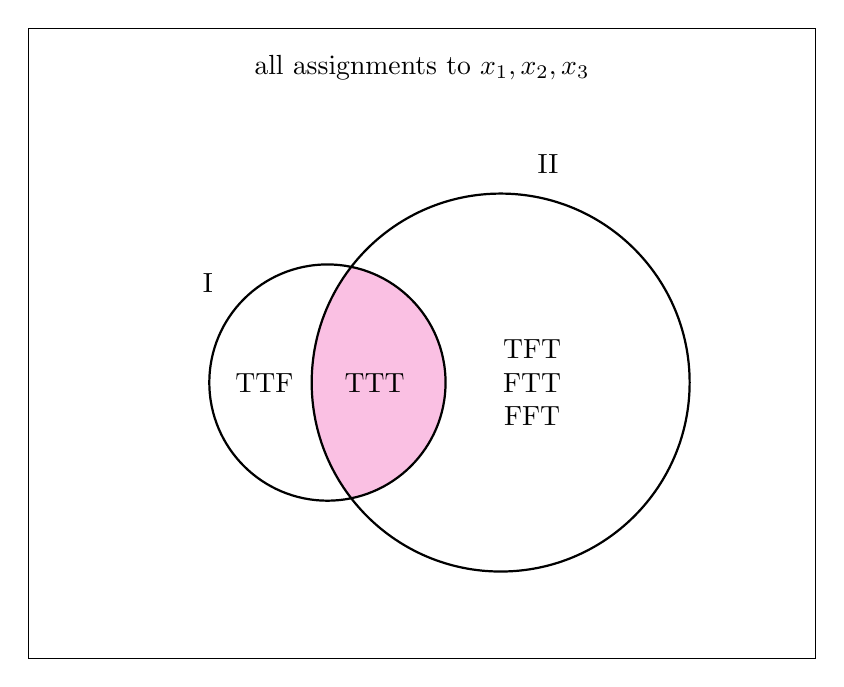
\begin{tikzpicture}
    \def\firstcircle{(180:1.2) circle[radius = 1.5]}
    \def\secondcircle{(0:1) circle[radius = 2.4]}

    \node at (155:3) {I};
    \node at (60:3.2) {II};

    \begin{scope}
      \clip \firstcircle;
      \fill[fill=Rhodamine!30] \secondcircle;
    \end{scope}
    \draw[thick] \firstcircle \secondcircle;

    \node at (180:2) {TTF};
    \node at (180:.6) {TTT};
    \node[align=center] at (0:1.4) {TFT \\ FTT \\ FFT};

    \draw (-5, 4.5) rectangle (5, -3.5);

    \node at (0, 4) {all assignments to $x_1, x_2, x_3$};
  \end{tikzpicture}
  \caption{An illustration of problems in Algorithm \ref{alg:2-conj}.}
  \label{fig:2-conj}
\end{figure}

The first problem is easy to fix; we simply replace line \ref{line:conj} in Algorithm \ref{alg:2-conj} to ``pick $i \in \{ 1, 2 \}$ \emph{proportional to the number of satisfying assignments for that conjunction}.'' For the second problem, we introduce the notion of \emph{rejection sampling}. Let $m$ be the number of conjunctions in $\varphi$. For each $i \in [m]$, let $A_i = \{ \bar x = (x_1, \ldots, x_n) : \text{$\bar x$ satisfies the $i^\text{th}$ conjunction} \}$. Consider the example illustrated in Figure \ref{fig:rej-samp}. In the shaded region in Figure \ref{fig:rej-samp}, each assignment is $3$ times more likely to be picked; therefore, we correct our algorithm by tossing a coin of bias $1/3$ to decide if to output the assignment. We summarize our final algorithm in Algorithm \ref{alg:unif-gen}.

\begin{figure}
  \centering
  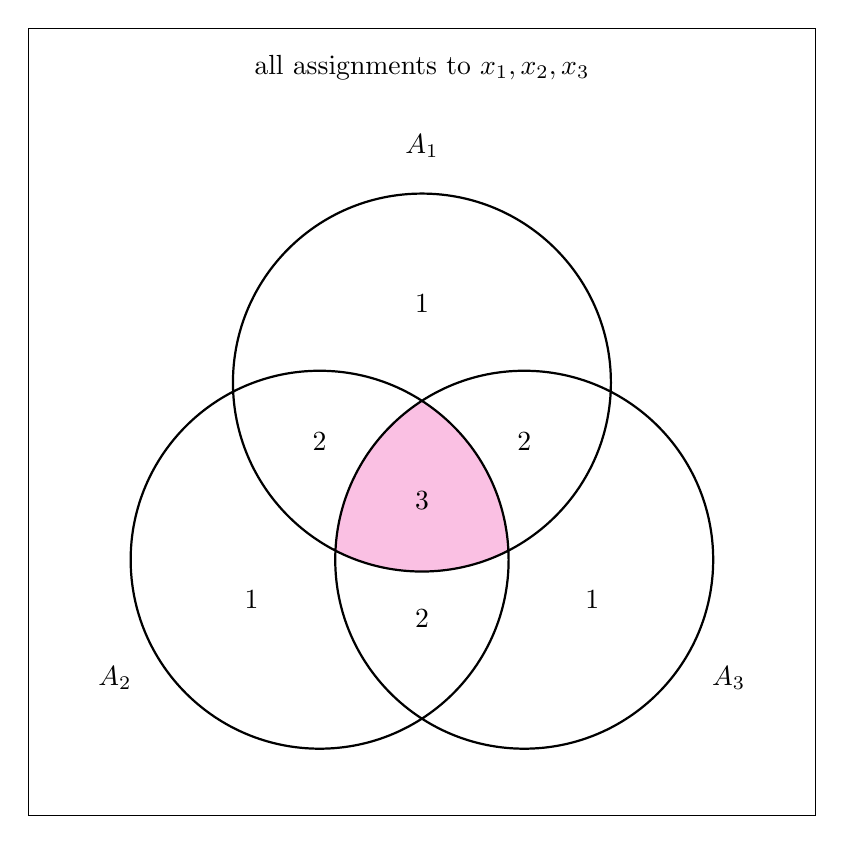
\begin{tikzpicture}
    \def\firstcircle{(90:1.5) circle[radius = 2.4]}
    \def\secondcircle{(210:1.5) circle[radius = 2.4]}
    \def\thirdcircle{(330:1.5) circle[radius = 2.4]}

    \node at (90:4.5) {$A_1$};
    \node at (210:4.5) {$A_2$};
    \node at (330:4.5) {$A_3$};

    \begin{scope}
      \clip \firstcircle;
      \clip \secondcircle;
      \fill[fill=Rhodamine!30] \thirdcircle;
    \end{scope}
    \draw[thick] \firstcircle \secondcircle \thirdcircle;

    \node at (270:1.5) {$2$};
    \node at (0:0) {$3$};
    \node at (150:1.5) {$2$};
    \node at (30:1.5) {$2$};
    \node at (90:2.5) {$1$};
    \node at (210:2.5) {$1$};
    \node at (330:2.5) {$1$};

    \draw (-5, 6) rectangle (5, -4);

    \node at (0, 5.5) {all assignments to $x_1, x_2, x_3$};
  \end{tikzpicture}
  \caption{An example for rejection sampling, where the number in each region indicates the number of conjunctions each assignment satisfies.}
  \label{fig:rej-samp}
\end{figure}

\begin{algorithm}
  \DontPrintSemicolon
  $A_i = \{ \bar x = (x_1, \ldots, x_n) : \text{$\bar x$ satisfies the $i^\text{th}$ conjunction} \}$ for each $i \in [m]$ \\
  \Repeat{success}{
    pick $i \in [m]$ with probability $|A_i|/\sum_{j = 1}^m |A_j|$ \\
    pick $\bar b \in A_i$ uniformly \\
    $t_{\bar b} \leftarrow |\{ j \in [m] : \bar b \in A_j \}|$ \CommentSty{// $t_{\bar b} \geq1$ since $\bar b$ satisfies $C_i$} \\
    output $\bar b$ with probability $1/t_{\bar b}$
  }
  \caption{Uniform generation for DNF, where the input is a DNF formula $\varphi = \bigvee_{i = 1}^m C_i$ and $C_i$ is a conjunction for each $i \in [m]$.}
  \label{alg:unif-gen}
\end{algorithm}

We show the uniformity of Algorithm \ref{alg:unif-gen}. For each $\bar b$ that satisfies $\varphi$,
\begin{align*}
  \PP\left[\text{$\bar b$ is output in round $i$}\right] &= \frac{1}{t_{\bar b}} \sum_{\substack{j \in [m] \\ \bar b \in A_j}} \PP[\text{pick $j$ in round $i$}] \cdot \frac{1}{\left|A_j\right|} \\
  &= \frac{1}{t_{\bar b}} \sum_{\substack{j \in [m] \\ \bar b \in A_j}} \frac{\left|A_j\right|}{\sum_{k = 1}^m \left|A_k\right|} \cdot \frac{1}{\left|A_j\right|} \\
  &= \frac{1}{t_{\bar b}} \sum_{\substack{j \in [m] \\ \bar b \in A_j}} \frac{1}{\sum_{k = 1}^m \left|A_k\right|} \\
  &= \frac{1}{\sum_{k = 1}^m \left|A_k\right|}.
\end{align*}
Hence, the probability that $\bar b$ is output in round $i$ is the same for all $\bar b$ satisfying $\varphi$, so the generation is uniform. Moreover, $\PP[\text{loop success}] \geq 1/\max t_{\bar b}\geq 1/m$, so $\EE[\text{\# loops until success}] \leq m$. This shows that Algorithm \ref{alg:unif-gen} runs in polynomial time in expectation.

\section{Counting Problems}

\begin{definition}
  Let $\shP$ denote the class of problems that count the number of accepting paths in a polynomial time nondeterministic Turing machines.
\end{definition}

\begin{definition}
  We say that a problem is \emph{$\shP$-complete} if
  \begin{enumerate}[label=(\alph*), itemsep=0pt]
    \item it is in $\shP$;
    \item every problem in $\shP$ has a polynomial time reduction to it.
  \end{enumerate}
\end{definition}

Let $\shSAT$ denote the problem that counts the number of assignments satisfying a Boolean formula $\varphi$. Then $\shSAT$ is $\shP$-complete. Similarly, let $\shDNF$ denote the problem that counts the number of assignments satisfying a DNF formula $\varphi$. Although $\DNF \in \Poly$, we show below that $\shDNF \not \in \Poly$. However, it turns out that $\shDNF$ is $\shP$-complete.

\begin{proposition}
  $\shDNF \not \in \Poly$.
\end{proposition}

\begin{proof}
  We show that if $\shDNF \in \Poly$, then $\CNF \in \Poly$. By De Morgan's law, a clause $\overline{A \vee B} = \overline{A} \wedge \overline{B}$, which is a conjunction. Therefore, Given a CNF formula $\varphi$ in $n$ variables, $\varphi$ is satisfiable if and only if $\overline \varphi$ (which is a DNF formula) has at most $2^n - 1$ satisfying assignments.
\end{proof}

\section{Approximate Counting}

\begin{definition} \label{def:fpras}
  A \emph{fully polynomial randomized approximation scheme (FPRAS)} for DNF is an algorithm which, given a DNF formula $\varphi$ and $\varepsilon > 0$, outputs $y \in \ZZ_+$ such that $z/(1 + \varepsilon) \leq y \leq z(1 + \varepsilon)$ with probability at least $3/4$ in time polynomial in $|\varphi$ and $1/\varepsilon$, where $z$ is the number of satisfying assignments to $\varphi$.
\end{definition}

In Problem Set 1 Problem 1, we shall show that Definition \ref{def:fpras} implies that an FPRAS runs in time polynomial in $|\varphi|$, $1/\varepsilon$ and $\log \delta$ if we replace the probability bound $3/4$ with $1 - \delta$.

\begin{proposition}
  If there exists an FPRAS for $\shSAT$, then $\SAT \in \BPP$.
\end{proposition}

\begin{proof}
  We give a probabilistic algorithm for SAT. Given a Boolean formula $\varphi$, we call the FPRAS on $\varphi$ with $\varepsilon = 1/2$ (or any constant); if the output of the FPRAS is positive, then output ``satisfiable''; else output ``unsatisfiable.''

  If $\varphi$ is satisfiable, then the number of satisfying assignments is at least $1$, so $y \geq 1/(1 + \varepsilon) > 0$, which impies that the algorithm outputs ``satisfiable.'' Otherwise, the number of satisfying assignments is $0$, so $y = 0$, which implies that the algorithm outputs ``unsatisfiable.''
\end{proof}

\end{document}
